%$Author: jlconlin $
%$Date: 2007-03-24 10:35:35 -0600 (Sat, 24 Mar 2007) $
%$Revision: 33 $
%$Id: ArnoldiMC.tex 33 2007-03-24 16:35:35Z jlconlin $
\documentclass[12pt]{article}
\usepackage{geometry}
\usepackage{amsmath}
\usepackage{setspace}
\usepackage[algo2e, ruled, linesnumbered]{algorithm2e}
\usepackage[usenames, dvipsnames]{color}
\usepackage{amsthm}
\usepackage{graphicx}

\SetKwComment{Comment}{$\triangleright$ }{}
\dontprintsemicolon

\newtheorem{theorem}{Theorem}
\newtheorem{coro}[theorem]{Corollary}

\author{Jeremy Conlin}
\title{Arnoldi's Method in Monte Carlo}

\begin{document}
\maketitle

\begin{abstract}
This document was written to help the author understand Monte Carlo Arnoldi's method.  There are mistakes and many assumptions are not explicitly stated.  USE AT YOUR OWN RISK! No warranty expressed or implied.
\end{abstract}

\section{Iteration}
One Arnoldi Iteration begins with sampling the fission source and tracking those particles with Monte Carlo transport.  This should be the only portion of this method that uses Monte Carlo transport.  The remainder should be the same as the deterministic method.

\subsection{Monte Carlo Transport}
The Monte Carlo portion begins by sampling from a fission source.  In this formulation, the fission source is a histogram source where some bins may have negative values.  The number of neutrons sampled from this distribution is constant between Monte Carlo cycles (although it doesn't have to be).  

After the neutrons are sampled, they are transported as in a traditional Monte Carlo Power Method calculation.  The neutrons create additional fission neutrons at every collision.  The number of fission neutrons added to the bank at each collision is dependent on the weight of the colliding neutron,
\begin{equation} \label{eq:num-fission}
    N = \left\lfloor\omega\left(\frac{\nu\Sigma_f}{\Sigma_t}\right) + \xi\right\rfloor\,,
\end{equation}
while the weight of the neutron is reduced as
\begin{equation}
    \omega = \omega'\left(\frac{\Sigma_s}{\Sigma_t}\right).
\end{equation}

A neutron is transported until it leaves the slab geometry or its weight becomes too small ($\omega < 0.2$) at which point, it plays Russian Roulette.  Currently, the survival probability is: $p_s = 0.8$, that is, 80\% of the time, the particle will be killed.  The weight of a surviving particle is increased as
\begin{equation}
    \omega = \omega'\frac{1}{p_s}.
\end{equation}

\subsubsection{Negative Weight Neutrons}
Arnoldi's method cannot guarantee you won't get negative sources.  More often than not, you will have negative sources.  So how can we deal with this?  What exactly is a negative fission source?  The answer isn't as difficult as it might first seem.  A particle sampled from a negative source has a negative weight.  Every time a negative weight neutron makes a score, it subtracts from the tally.  

We can envision our transport as two independent Monte Carlo transport problems; one whose source is the positive portion of the PDF and the other source is the absolute value of the negative PDF.  Both sources are sampled, transported, tallied and binned.  The negative source is then subtracted from the positive source in each bin.  

The total number of particles transported is
\begin{equation}
    h = N_p + N_n,
\end{equation}
where $N_p$ is the number of neutrons from the positive PDF and $N_n$ is the number of neutrons from the negative PDF.  The ratio of the number of positive weight particles to negative weight particles is ratio of the probability of picking a positive weight particle to the probability of picking a negative weight particle,
\begin{equation}\label{eq:PDFprob}
    \frac{N_p}{N_n} = \frac{\int{Q_p}}{\int{Q_n}}\,.
\end{equation}

So what do we do with negative weight particles?  Using Eq. \ref{eq:num-fission} a negative weight particle will \emph{never} add a neutron to the fission bank.  I suspect what we need to do is modify Eq. \ref{eq:num-fission} to use the absolute value of the weight; 
\begin{equation}
    N = \left\lfloor|\omega|\left(\frac{\nu\Sigma_f}{\Sigma_t}\right) + \xi\right\rfloor\,
\end{equation}
I also need take into account the sign of the particle's weight (but not it's magnitude) when binning a fission bank.  

Similarly when I decide whether or not I should play Russian Roulette, I need to see if the absolute value of the weight is less than some cutoff.
\normalcolor

\subsection{``Matrix-ify'' Fission Bank}
Monte Carlo transport returns a new fission bank---a collection of fission neutrons---that traditionally would have been used directly for the next cycle.  With Arnoldi's Method we need to take this fission bank and turn it into something like a vector.  This vector must be able to be multiplied by a scalar and added and subtracted to other vectors.

We have chosen to turn our fission banks into vectors by binning or making a histogram out of the fission neutrons.  The value or height in each bin represents the number of fission neutrons in each geometrical bin.  The histogram is normalized and the bin values become the elements of the vector.

\subsubsection{Fission Source Normalization}
I don't understand why, but this is how you normalize the fission source, immediately after it has been binned, before you apply Arnoldi to it,
\begin{equation}
    q_{k+1} = q_{k+1}\frac{1}{N}\int{\left|q_k\right|}.
\end{equation}
By normalizing in this way, the bins are the probabilities of a fission occurring in that bin \emph{per source particle}.

\begin{figure}[h]
    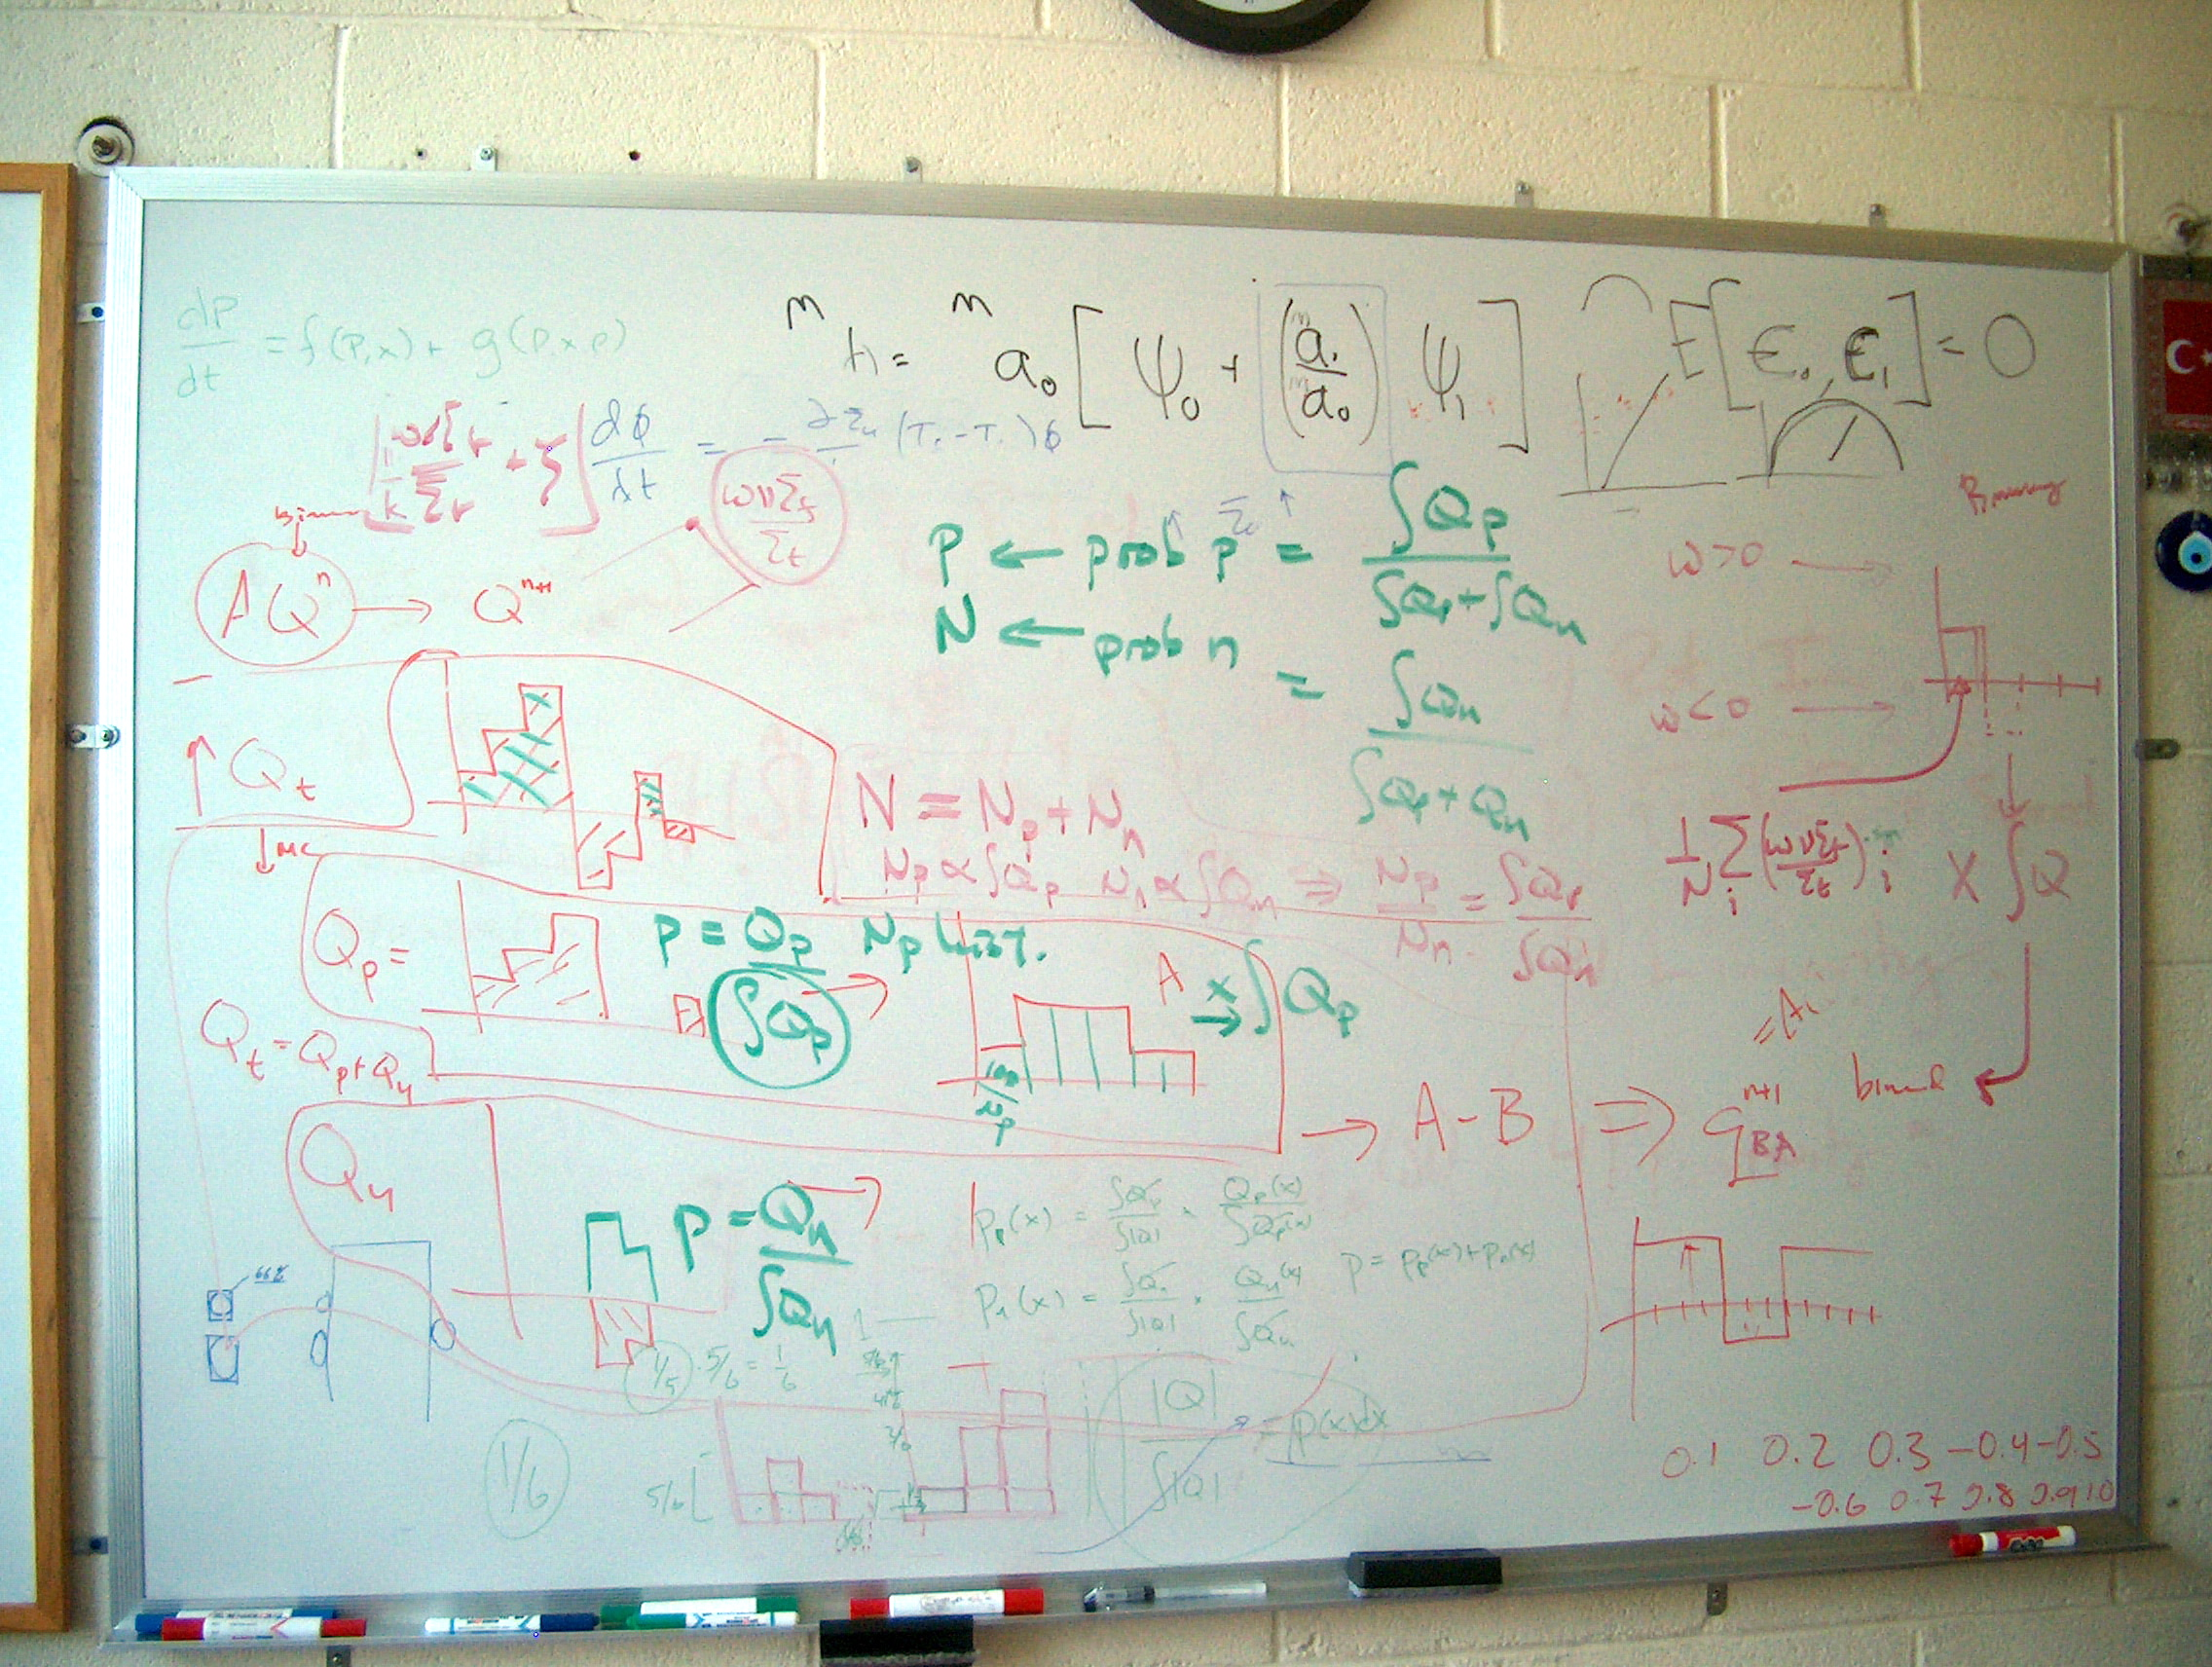
\includegraphics[width=6in, keepaspectratio]{Whiteboard.jpg}
\end{figure}

\subsection{Orthogonalize} \label{sec:Orthogonalize}
In the $k^{th}$ iteration, the operation 
\begin{equation}
    q_{k+1} = Aq_k,
\end{equation}
is performed where $A$ is what I will call the Monte Carlo operator, and the $q$'s are fission sources.  We already have an orthonormal set of fission sources $\{q_1, q_2, \dots, q_k\}$ which span the Krylov subspace.  For each of these previously generated sources, we perform two calculations,
\begin{subequations} \label{eq:Orthogonalize}
\begin{gather} 
    h_{j,k} = \left<q_j, Aq_k\right> = \left<q_j,q_{k+1}\right> \\ 
    q_{k+1} = q_{k+1} - h_{j,k}*q_j,
\end{gather}
\end{subequations}
to orthogonalize $q_{k+1}$ and also to create an upper hessenberg matrix, $h$, which has the same eigenvalues as the linear operator $A$ we are investigating.

Applying Eqs. \ref{eq:Orthogonalize} for every previously generated source ($q_j$) on the current source, $q_{k+1}$ will make $q_{k+1}$ orthogonal to all $q_j$'s.  Now all that remains is to normalize $q_{k+1}$ and add one more entry to our upper hessenberg matrix;
\begin{subequations}\begin{gather}
    h_{k+1,k} = \left<q_{k+1},Aq_{k}\right> = \left<q_{k+1},q_{k+1}\right> = \left\|q_{k+1}\right\|_2 \\
    q_{k+1} = q_{k+1}/h_{k+1,k}.
\end{gather}\end{subequations}

\subsection{Eigenvalues}
The Arnoldi formulation proves that our upper hessenberg matrix, $h$, and our matrix (or linear operator) of interest, $A$, are similar and therefore have the same eigenvalues.  Finding the eigenvalues of $h$ is easy because $h$ is small compared to $A$ and also because it is upper hessenberg.  Therefore, to find the eigenvalues of $A$, we create $h$ through the orthogonalization process defined in section \ref{sec:Orthogonalize} and then use our favorite eigenvalue calculator.

\subsection{Eigenvectors}
Even though $h$ and $A$ are similar, this doesn't guarantee they have the same eigenvectors.  In fact they won't because the dimension of the eigenvectors of $h$ will be much smaller than those of $A$.  

The eigenvectors of $A$ associated with the eigenvalues calculated from the similar matrix $h$, can be calculated as a linear combination of the orthonormal vectors, $q_j$.  The expansion coefficients for eigenvector $i$ are the elements of the $i^{th}$ eigenvector of $h$. 

\subsection{Residual}
The residual norm gives some indication of how close we have converged upon our solution.  Saad (1992) shows that the residual norm is just the last component of the eigenvector $y_i^{(m)}$ multiplied by $h_{m+1,m}$.  This works well in the deterministic calculation, but I'm not sure it will works for all cases in the Monte Carlo calculation.

Suppose, if you will, that you have a point source in a---nearly---infinite medium.  The orthonormal vectors calculated will have non-zero elements in the middle few bins, and zeros elsewhere.  When calculating the eigenvector of the Monte Carlo operator, the outer elements of the eigenvector will also be zero.  For an infinite medium problem, the residual will be zero immediately.  

Saad does say that the residual norms are ``not always indicative of actual errors'', but ``are quite helpful in deriving stopping procedures.''  For Monte Carlo applications of Arnoldi's Method, it seems clear that this simple calculation of the residual may give incorrectly small values and we might stop prematurely.

\section{Uncertainty}
Once the eigenvalue has been found, we must be able to place an uncertainty about it.  Our Matrix-Vector product is stochastic and our uncertainty should be in a form of standard deviation.

\section{Restarting}
One can restart Arnoldi's method after some number of iterations to reduce the memory requirements and the number of orthogonalization steps.  After a predetermined number of iterations, the simulation is stopped, the eigenvector of interest is calculated and this eigenvector (e.g. fission source) is used as the initial guess for an entirely new Arnoldi process.

\section{Preliminary Results}
I have a working version of Monte Carlo Arnoldi's method.  In this section, I present some arguments to give confidence to the results received.  

\subsection{Uncertainty}
Currently we have no direct way of determining the uncertainty of a Monte Carlo Arnoldi simulation.  To get a rough estimate, I ran 50 simulations and calculated their average and variance/standard deviation.  The geometry was discretized into 10 bins.  I ran this series of simulations five times with 1000 histories per iteration and five times with 10,000 histories per cycle.  With 1000 histories per iteration the standard deviation was 0.01; with 10,000 histories per cycle the standard deviation was 0.004.

\subsection{Residual}
In Arnoldi's method, we can calculate the residual norm, a simple measure of the convergence of the calculated eigenvalues to the true eigenvalues.  Once the residual is sufficiently small iteration stops.  In deterministic Arnoldi's method, this is a good way to determine stopping procedures. 

When investigating the Monte Carlo version of Arnoldi's method it would be nice to see the residual norm decrease as a function of Arnoldi iteration just as the deterministic does, but with the stochastic noise.  In Figure \ref{fig:Residual} the residual norm for both deterministic and Monte Carlo simulations are shown.  The deterministic simulation is a $1000 \times 1000$ diagonal matrix with the vector $[1,2,\ldots, 1000]$ on the diagonal.  The Monte Carlo simulation had slab geometry with half-width 0.5 mfp and discretized into 10 spatial bins.  Although the residual of the Monte Carlo simulation doesn't decrease as much as the deterministic residual, it does have the same trend of decreasing.

In my (limited) experience, the dominant eigenvalue is determined to machine precision before the residual is sufficiently low.  I believe this is due to the stochastic nature of Monte Carlo methods.  The residual hovers around $10^{-3}$ until the Krylov subspace has been spanned and then immediately drops to $10^{-13}$ or smaller.  The maximum number of iterations before the subspace has been spanned is equal to the number of spatial bins.  A simulation with 100 spatial bins would span the Krylov subspace in at most 100 iterations, but the eigenvalue is found---to within machine precisions---in about 50 iterations.
\begin{figure}[h]\centering
    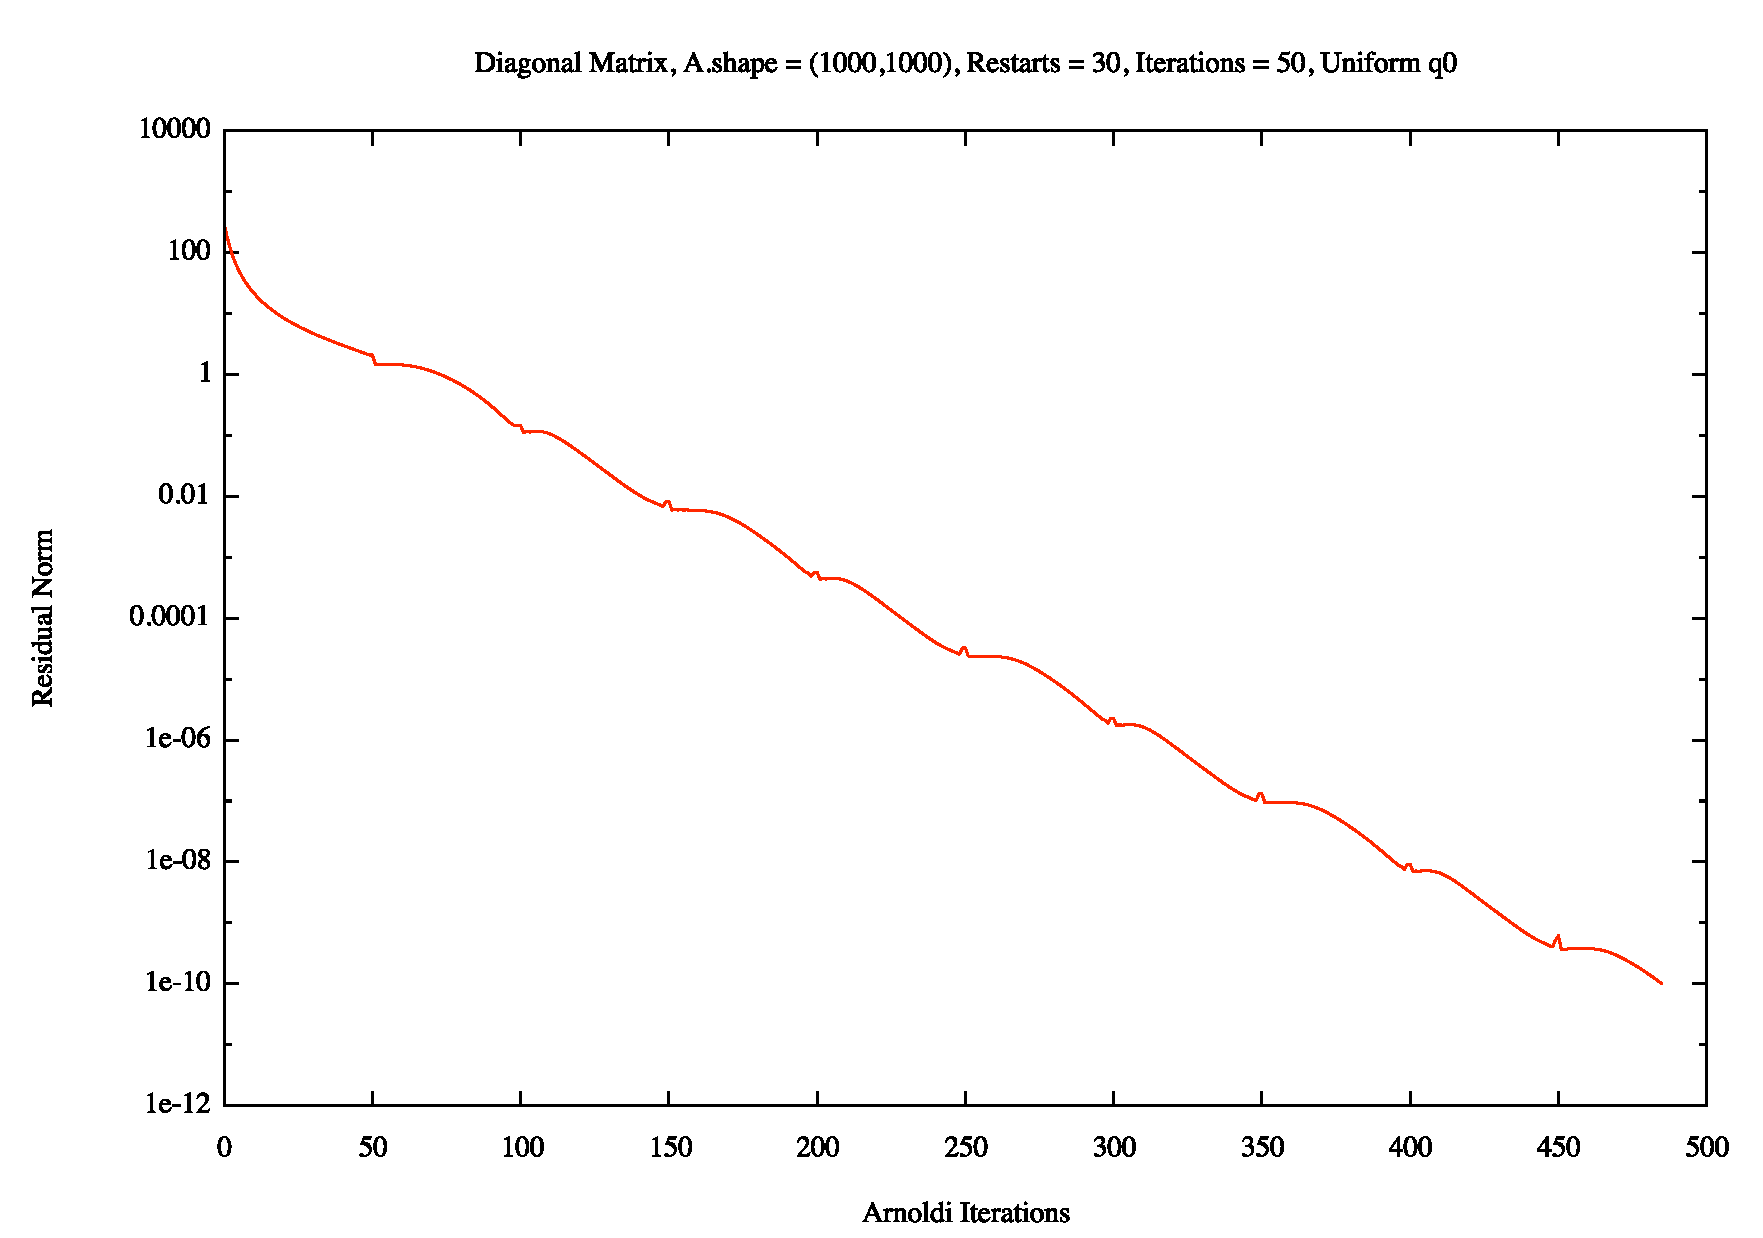
\includegraphics[width=5in, keepaspectratio]{ArnoldiDtmResidual.pdf}
    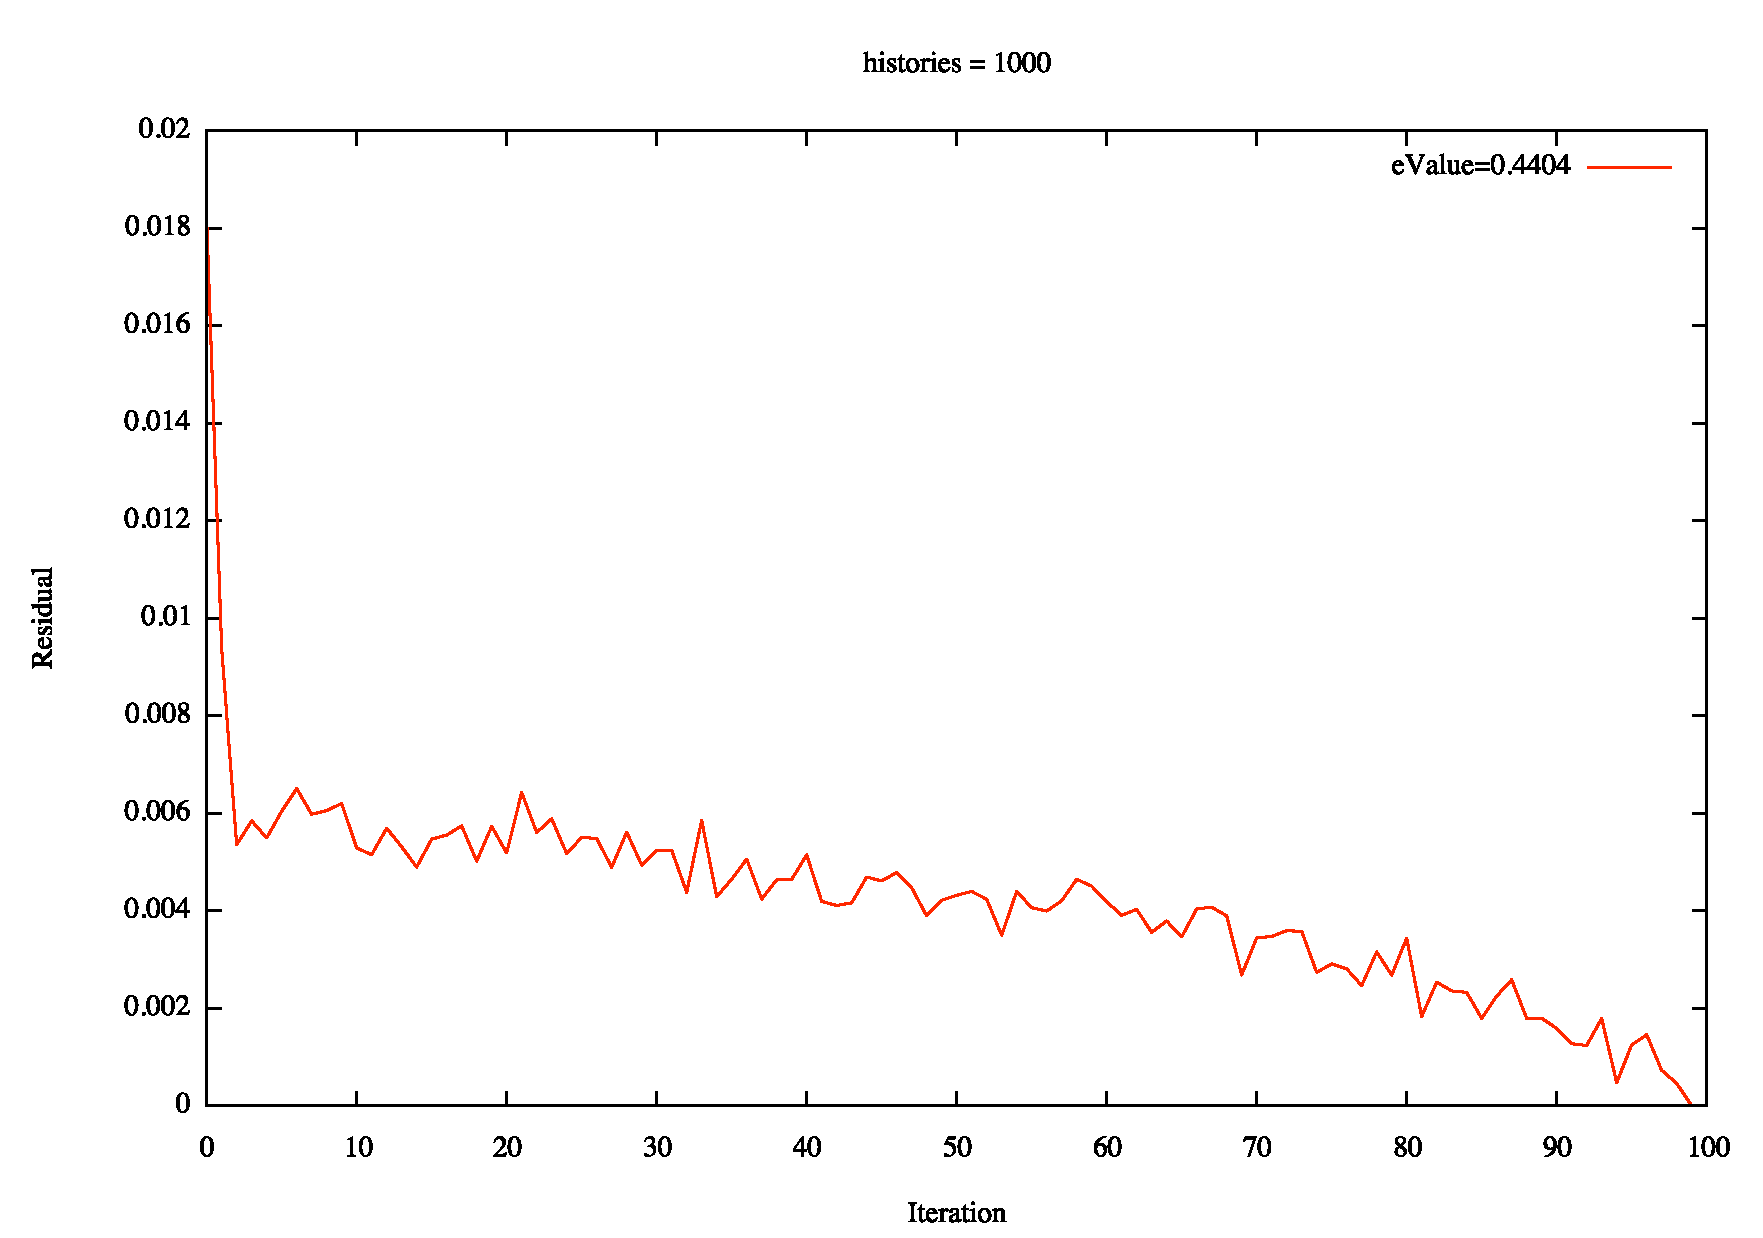
\includegraphics[width=5in, keepaspectratio]{ArnoldiMCResidual.pdf}
    \caption{Residual norm as a function of the number of Arnoldi Iterations.  Top figure is Deterministic and the ``blips'' are when Arnoldi restarted.  The bottom figure is Monte Carlo.}
    \label{fig:Residual}
\end{figure}


\subsection{Eigenvalue and Timing Comparisons}
Comparing Monte Carlo Arnoldi's method to a traditional Power method is difficult.  First of all, we don't yet have a good way of determining the uncertainty in the eigenvalue for Arnoldi's method.  Second, it may be difficult to determine when the Power method has converged.  

In this illustration I have used 1000 histories per iteration/cycle.  As indicated previously, this is roughly an uncertainty of 0.01 in Arnoldi's method.  The Power method used 20 inactive cycles and the uncertainty was comparable with that of Arnoldi's method.  The geometry was slab geometry with varying half-width.  In both Arnoldi's method and the Power method, the fission source was discretized into 10 spatial bins.  I show the results in Table \ref{tbl:Timing} where the results are compared with ``benchmark'' results from Martin and Duderstadt\footnote{William R. Martin and James J. Duderstadt, \emph{Nuclear Science an Engineering}, \textbf{62}, 371-390 (1970)}.

\begin{table}[h]\centering
    \caption{Eigenvalue and timing comparisons.}
    \label{tbl:Timing}
    \vspace{11pt}
    \begin{tabular}{|c|c|c|c|c|c|} \hline
        Half width [mfp] & M\&D & MC Arnoldi & time [s] & MC Power & time [s] \\ \hline
        0.5  & 0.448278 & 0.4520 & 2.1 & 0.4492 $\pm$ 0.011 & 4.8  \\ \hline
        1.0  & 0.643416 & 0.6438 & 2.5 & 0.6423 $\pm$ 0.019 & 5.7  \\ \hline
        5.0  & 0.952601 & 0.9545 & 4.2 & 0.9581 $\pm$ 0.024 & 8.6  \\ \hline
        10.0 & 0.985831 & 0.9899 & 4.8 & 0.9950 $\pm$ 0.025 & 9.0  \\ \hline
        30.0 & ---      & 1.0049 & 4.7 & 1.0078 $\pm$ 0.019 & 9.4  \\ \hline
    \end{tabular}
\end{table}

With this comparison it seems that one can accurately calculate the eigenvalue using a Monte Carlo version of Arnoldi's method.  From these results, it looks like Arnoldi's method is faster than the Power method, however it will take a more careful and detailed tests to make a definite decision.

\subsection{Eigenvector}
I am still working out the details of calculating the dominant eigenvector associated with the (correct) eigenvalue calculated.  In the tests shown in Table \ref{tbl:Timing} I can get the correct shape---roughly cosine---for each test.  Sometimes the eigenvector comes out upside-down.  This isn't too much of a problem since we know the eigenvector is only unique times a multiplicative constant; this constant could be -1.  Almost always, the eigenvector is negative at the edges of the slab.  This is more cause for concern; we know the eigenvector (the flux) must be zero or positive everywhere.  What then is to be done with negative components of the eigenvector?  I have plotted two resulting eigenvectors in Figure \ref{fig:Vector}, both were calculated with 10,000 histories per iteration.


\begin{figure}[h]\centering
    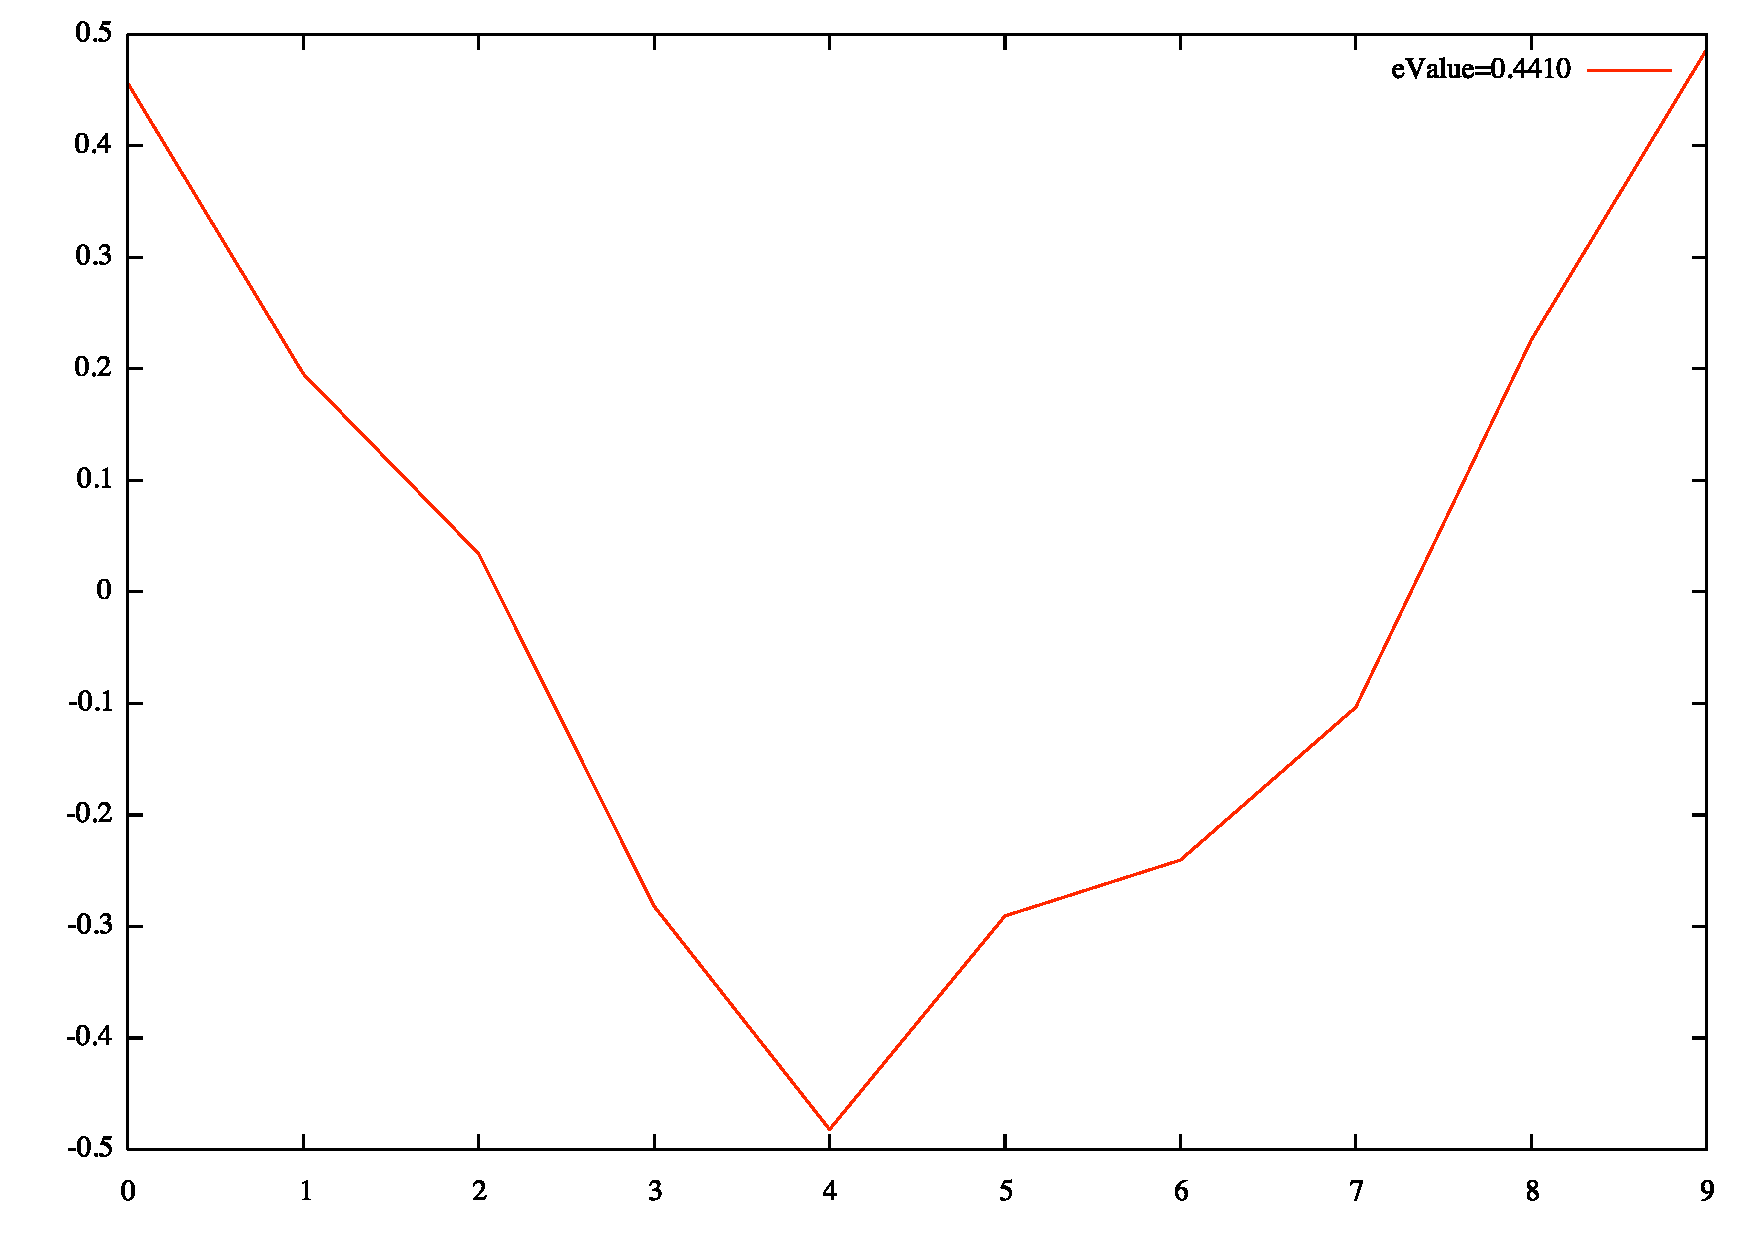
\includegraphics[width=5in, keepaspectratio]{NegativeEigenvector.pdf}
    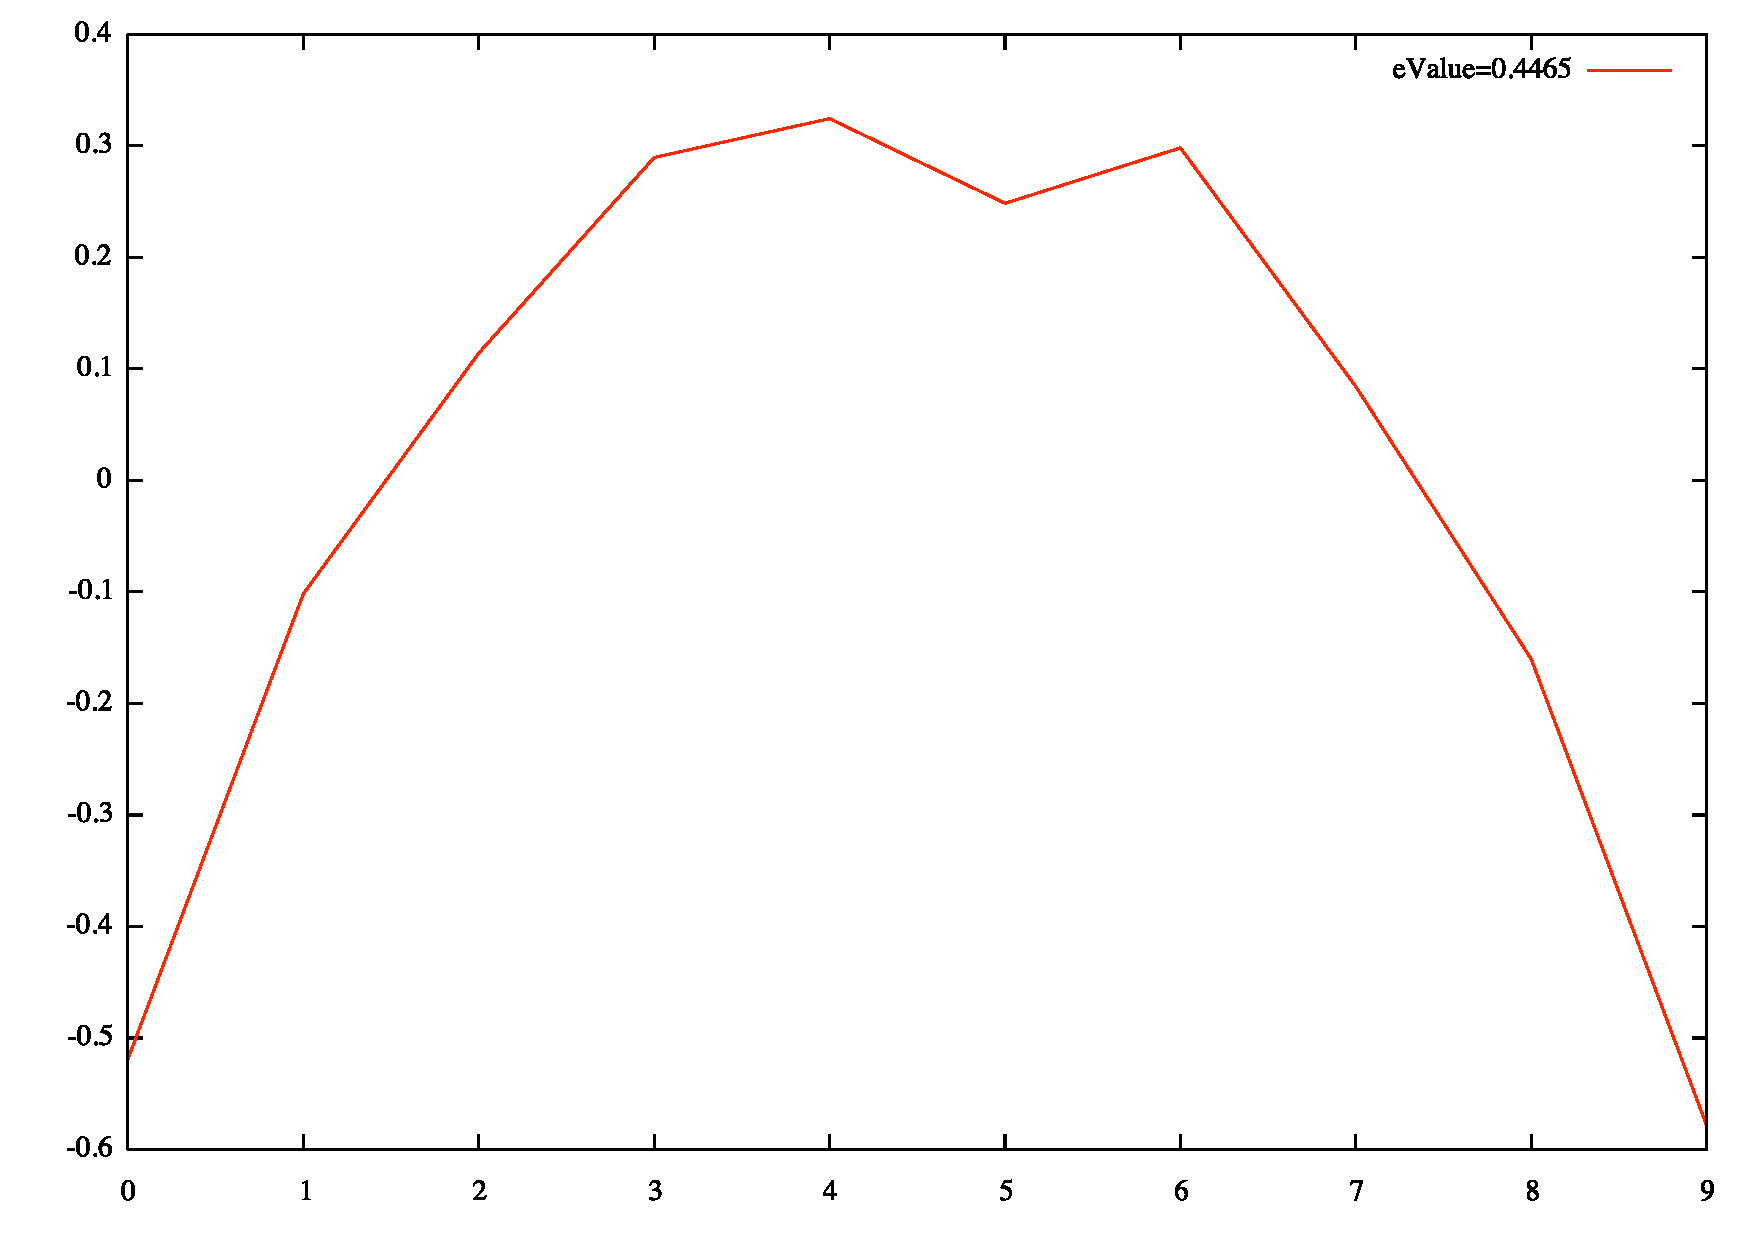
\includegraphics[width=5in, keepaspectratio]{PositiveEigenvector.pdf}
    \caption{Eigenvector from two separate Monte Carlo Arnoldi simulations showing potential problems.}
    \label{fig:Vector}
\end{figure}


\newpage
\section{Algorithms}
\begin{algorithm2e}
    \SetVline
    \caption{Deterministic Arnoldi Process (freely borrowed from Watkins(2002))}\label{alg:DtmArm}
    $q_1 = q/\left\|q\right\|_2$ \;
    \For{$k=1,\ldots,m-1$}{
        $q_{k+1} \gets Aq_k$\;
        \For(\Comment*[f]{Orthogonalize}){$j=1, \ldots, k$}{ 
            $h_{jk} \gets \left<q_j,q_{k+1}\right>$\;
            $q_{k+1} \gets q_{k+1} - q_jh_{jk}$}
        $h_{k+1,k} \gets \left\|q_{k+1}\right\|_2$\;
        \If(\Comment*[f]{Span \{$q_1, \ldots, q_k$\} is invariant under $A$}){$h_{k+1,k} = 0$}{
            quit.}
        $q_{k+1} \gets q_{k+1}/h_{k+1,k}$\;
    }
\end{algorithm2e}

\begin{algorithm2e}
    \SetVline
    \caption{Deterministic Arnoldi Process, Python Style}\label{alg:DtmArnPy}
    \For(\Comment*[f]{$I$ = \# of Arnoldi Iterations.}){$k=1, \ldots, I+1$}{
        $q \gets AQ_{k-1}$\Comment*[f]{$(k-1)^{\textrm{st}}$ or last column of $Q$} \;
        \For{$j=1, \ldots, k+1$}{
            $h_{j-1,k-1} = \left<Q_{j-1},q\right>$ \Comment*[f]{$(j-1)^{\textrm{st}}$ column of $Q$} \;
            $q \gets q - Q_{j-1}*h_{j-1,k-1}$}
        $h_{k,k-1} \gets \left\|q\right\|_2$ \;
        $q = q/h_{k,k-1}$ \;
        \If(\Comment*[f]{Residual too small.}){$h_{k,k-1}*y_m < 10^{-10}$}{
            quit\Comment*[f]{See Saad 1992 p.175-76.}}
        $Q = \left[Q|q\right]$ \Comment*[f]{Append $q$ as last column of $Q$}}
\end{algorithm2e}

\begin{algorithm2e}
    \SetVline
    \caption{Monte Carlo Arnoldi Process}\label{alg:MCArnoldi}
    \For{$k=1, \ldots, iterations + 1$}{
        $q = AQ_k = \ldots$ \Comment*[f]{Monte Carlo portion} \;
        $q = \left(q/N\right)\int{\left|Q\right|}$ \Comment*[f]{Monte Carlo normalization} \;
        \For{$j=1, \ldots, k+1$}{
            $h_{j-1,k-1} = \left<Q_{j-1},q\right>$ \;
            $q = q - h_{j-1,k-1}*Q_{j-1}$}
        $h_{k,k-1} = \left\|q\right\|_2$ \Comment*[f]{Arnoldi normalization}\;
        $q = q/h_{k,k-1}$ \;
        Calculate eigenpairs\;
        Sort eigenpairs\;
        \If(\Comment*[f]{Residual too small.}){$h_{k,k-1}*y_m < 10^{-10}$}{
            quit Arnoldi.  Start Power Method.\Comment*[f]{See Saad 1992 p.175-76.}}
        $Q = \left[Q|q\right]$ \Comment*[f]{Append $q$ as last column of $Q$}}
\end{algorithm2e}

\end{document}
